\begin{center}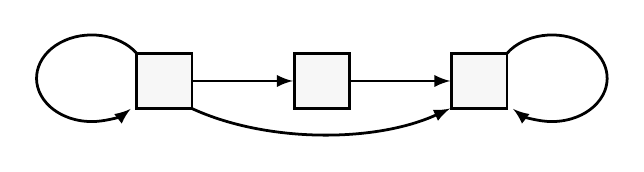
\begin{tikzpicture}
 [line width=1pt, bend angle=45,
 sq/.style={rectangle,inner sep=3pt, minimum size=7mm,
fill=black!3,draw=black}]
\node[sq] (dnode) at (0,0) {$\cchard$};
\node[sq] (fnode) at (2,0) {$\ccharf$};
\node[sq] (bnode) at (4,0) {$\ccharb$};
\draw[-latex] (dnode) -- (fnode);
\draw[-latex] (fnode) -- (bnode);
\draw[-latex] (-0.35,  0.35) arc(35:315:0.7cm and 0.55cm);
\draw[-latex] ( 4.35,  0.35) arc(145:-135:0.7cm and 0.55cm);
\draw[-latex] ( 0.35, -0.35) arc(230:310:2.55cm and 1.4cm);
\end{tikzpicture}\end{center}